\subsection{The Gilbert Normalizer}

I think this circuit is not to be known for the exam but it's way too elegant not to look at. Let's keep it quick:

\begin{figure}[H]
    \centering
    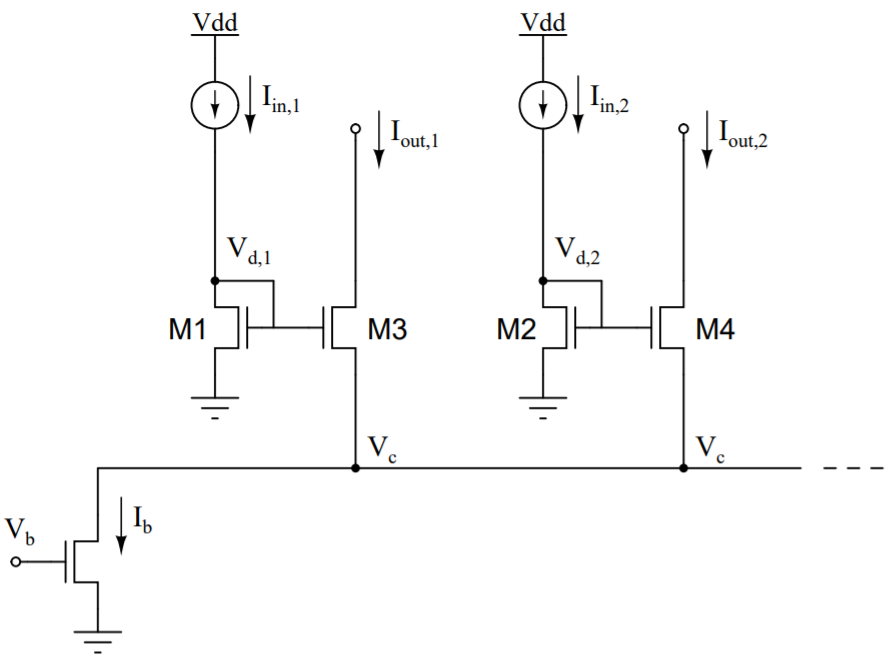
\includegraphics[width=0.6\linewidth]{../../Figures/Gilbert_Normalizer.PNG}
    \caption{Gilbert Normalizer circuit. Adapted from Lecture notes.}
    \label{fig:Gilbert_Normalizer}
\end{figure}

We assume subthreshold and saturation in all transistors: 

Because of Kirchoff's current law, the sum of currents flowing through each branch $I_{out_j}$ must be equal to $I_b$: 
Let's now note some things about $I_{in}$ and $I_{out}$ relationship, which is just driven by a current mirror arrangement. 

\begin{equation}
    I_{in_i} = I_0 e^{\frac{\kappa V_d_i}{U_T}}
\end{equation}
\begin{equation}
    I_{out_i} = I_0 e^{\frac{\kappa V_d_i}{U_T} - \frac{\kappa V_c}{U_T}} = I_{in}e^{\frac{\kappa V_c}{U_T}}
\end{equation}
\begin{equation}
    \mathrm{Since \ } I_b = \sum_{j}^{}I_{out_j}
\end{equation}
\begin{equation}
    \mathrm{We \ can \ write: }\ I_{out_i} = I_b \frac{I_{in_i}}{\sum_{j}^{}I_{in_j}}
\end{equation}

Hence implementing some kind of normalization of all $I_{out_i}$ flowing. Pretty cool!